\section{Horizontale Ausrichtung}
	
    Um die Abwurfeinheit zum Zielkorb auszurichten, wird ein verstellbarer Mechanismus benötigt, 
    mit einer sehr hohe Genauigkeit. Der Drehpunkt befindet sich unter den Beschleunigungsrädern, 
    damit die Position des Abwurfes im Zentrum des Spielfeldes bleibt. Die Drehbewegung erfolgt 
    mittels eines Schrittmotores. Die Ausführung des Schrittmotores ist sehr flach gewählt, damit 
    der Schwerpunkt der ganzen Konstruktion auch tiefer gelegt werden kann. Dies ist notwendig, 
    damit die ganze Ballmaschine eine grössere Stabilität aufweist. Der Schrittmotor kann eine 
    Haltemoment von 0.083\si{\newton\meter} halten. Dies ist genügend gross, um die ganze 
    Abwurfeinheit in der gewünschten Zeit zu bewegen und bei der Position zu halten. Durch den 
    Schrittmotor kann eine sehr genaue Ansteuerung vorgenommen werden. Der Schrittmotor wird in der Abwurfeinheit angebracht und treibt ein Ritzel an, welches in einen Zahnkranz in der Grundplatte 
    eingreift. Die Grundplatte besteht auch aus einem Kreissegment von ??55\si{\degree}?? 
    mit einem Zahnrad vom Modul 1. Das Ritzel am Motor besteht aus 32 Zähnen. Es ist aus einer 
    6\si{\milli\meter} dicken MDF\footnote{mitteldichte Faserplatte} gelasert worden, damit es auf 
    das die Motorenachse aufgepresst werden konnte. Dies ist mit Acrylglas nicht möglich da dieses 
    Material zu spröde ist. Dadurch kann die Abwurfeinheit gedreht werden. Dies ist in Abbildung 
    \ref{abb:Ausrichteinheit} ersichtlich. Damit die Bauhöhe nicht zusätzlich 
    vergrössert wird, ist der Zahnkranz in die Bodenplatte integriert. Um die Drehachse ist ein Kreis 
    mit dem Durchmesser der Breit vom Abwurfmechanismus integriert worden, welcher eine Abstützung 
    der ganzen Ballmaschine dient. 
    Damit der Schrittmotor keine hohes Drehmoment aufweisen muss, sind am Ende des Wurfmechanismus 
    zwei Kugellager angebracht, welche die Drehbewegung übernehmen. Dadurch ist die Reibung bei der 
    Drehbewegung sehr klein. Die Lagerung erfolgt im Drehzentrum durch eine Hülse.
    \begin{figure}[h!]
    	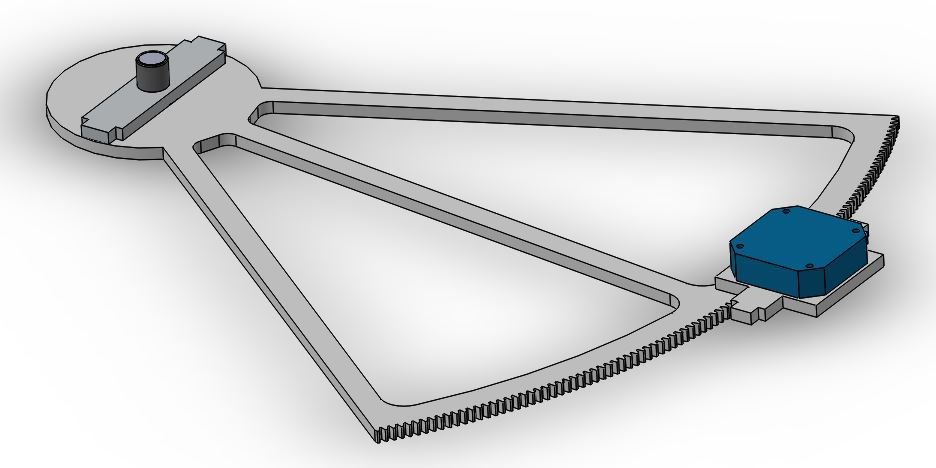
\includegraphics[width=0.8\textwidth,clip,trim=0mm 2mm 0mm 7mm]
    	{Enddokumentation/Bilder/Ausrichteinheit.jpg}
    	\centering
    	\caption{Ansicht der Ausrichteinheit}
    	\label{abb:Ausrichteinheit}
    \end{figure}
	%
    \subsection{Ansteuerung Steppermotor}
    \label{sec:StepperAnsteuerung}
        Die Ansteuerung des Stepper-Motors erfolgt über die entwickelte Hardware der PREN-ET-Gruppe. 
        Dieses Board kann direkt auf das Freedom-Board aufgesteckt und über die Konsole bedient 
        werden. Die gesamte Dokumentation dazu ist im Anhang \ref{apx:} angefügt. 
        
        \subsubsection{Auflösung}
        \label{sec:Aufloesung}
            Eine Umdrehung des Steppers benötigt 200 Vollschritte. Das Stepper-Board ist so konfiguriert, 
            dass $1:128$ Microstepping verwendet wird. Das gewählte Übersetzungsverhältnis vom 
            Stepper ist $1:28$ und somit ergeben sich die folgenden Auflösungen:
            \begin{equation}
                128 \cdot 200 \cdot 28 = 716'800\frac{\text{Microsteps}}{360\si{\degree}}
            \end{equation}
            \begin{equation}
                \frac{365\si{\degree}}{716'800} = 509 \cdot 10^{-6}\frac{\si{\degree}}{\text{Microsteps}}
            \end{equation}
            \begin{equation}
               \frac{1\si{\degree}}{509 \cdot 10^{-6}\frac{\si{\degree}}{\text{Microsteps}}} = 1963.8\frac{\text{Microsteps}}{\si{\degree}}
            \end{equation}
            